\documentclass[article]{memoir}
\setlrmargins{*}{*}{1}
\checkandfixthelayout
\usepackage[]{amssymb, amsthm, amsmath} 
\usepackage[]{mathtools} 
\usepackage[]{palatino} 
\usepackage[]{eulervm} 
\usepackage[]{graphicx} 
\usepackage[]{subcaption} 

\usepackage[]{minted} 
\usemintedstyle{friendly}
\usepackage[]{hyperref} 
\usepackage[capitalize, noabbrev]{cleveref} 

\newcommand{\x}{\mathbf{x}}
\newcommand{\f}{\mathbf{f}}
\newcommand{\R}{\mathbb{R}}
\renewcommand{\t}{\mathbf{t}}
\renewcommand{\c}{\boldsymbol{c}}
\newcommand{\A}{\boldsymbol{A}}
\newcommand{\B}{\boldsymbol{B}}
\newcommand{\G}{\boldsymbol{G}}
\newcommand{\tu}{\boldsymbol{\tau}_u}
\newcommand{\tv}{\boldsymbol{\tau}_v}
\renewcommand{\b}{\boldsymbol{b}}
\renewcommand{\S}{\mathcal{S}}


\title{\textsc{Assignment 4 \\ 
               MATINF4170 \\
       Spline Methods}}

\author{Ivar Haugal{\o}kken Stangeby}
\date{\today}

\begin{document}

\maketitle

\tableofcontents*

\chapter{Least square spline approximation}

In this assignment, we are to model a heart using cross sectional contour data
and least squares approximation. Before we start dealing with the specifics of
the heart model, we first recall the least squares approximation problem.
Being a generalization of the scalar version, we only go through the parametric
least squares approximation, as that is what we will employ in this assignment.

\section{Parametric curves}
\label{sec:para_curves}
Assume we are given a set of data on the form \((u_i, \x_i)_{i = 1}^{m}\),
where the \( u_i \in \R \) are the \emph{parameter values}, and the \( \x_i \)
are points in \( \R^d \) for some \( d \geq 1 \). Moreover, we fix a spline
space \(\S \coloneqq \mathbb{S}_{p, \t}\) for some knot vector \(\t\) and some
non-negative degree \( p \).  We set \( n \coloneqq \dim(\S)\).  We seek the
spline function \( f \) in the spline space \(\S\) that \emph{minimizes} the
squared error, i.e., 
\begin{equation} 
    \label{eq:least_squares_problem}
    f = \min_{g \in \S} \sum^{m}_{i=1} w_i (\x_i - g(\x_i))^2,
\end{equation}
where the \(w_i\)s are specified weights. This can be reformulated in linear
algebra terms as
\begin{equation}
    \label{eq:least_quares_linalg}
    \min_{\c \in \R^n} \| \A\c - \b \|^2, 
\end{equation}
where the matrix \( \A \in \R^{m, n} \) is given by \( a_{i, j} =
\sqrt{w_i}B_j(\x_i) \) and the vector \( \b \in \R^m \) is given by \( b_i =
\sqrt{w_i}\x_i \).

Under the assumption that \( m \geq n \), we can find the spline coefficients
of \( f \) by solving the linear system
\begin{equation}
    \notag
    \A^T\A\c = \A^T\b.
\end{equation}

\section{Parametric surfaces}

Finding the least squares approximation to a parametric surface is completely
analogous to the parametric curve case. Here we are instead dealing with tensor
product spline spaces \(\S \coloneqq \S_1 \otimes \S_2\).%
%
\footnote{This of course generalizes to the multi-variate case where the tensor
product spline space is \( \S = \S_1 \otimes \dots \otimes \S_k.\)}
%
The difference then lies in the data set, where we are given two sets of
parameter values, i.e., the data set is of the form \((u_i, v_j, \x_{i,j})_{i,
j}^{m_1, m_2}\). The linear system to solve is then
\begin{equation}
    \notag
    \A^T\A\c \B^T\B = \A^T\G\B, 
\end{equation}
for matrices similar to those in the curve case.

\chapter{Modelling cross sections of a heart.}
\label{sec:spline_representation_of_heart_contour_curves}

We are supplied with a collection of nine data sets, each on the form \(\x_i =
(x_i, y_i, z_i) \) for \( i = 1, \dots, m_j \) where \( m_j \) denotes the
number of data points for the \(j\)th data set. We step through the process
for a fixed \( j \).

\paragraph{Parametrization:}
In order to apply least squares spline approximation to data set \( j \), we
first need to find a suitable parametrization of the data. In this assignment
we chose the chord length parametrization, in general given as
\begin{equation}
    \notag
    u_i = u_{i-1} + \|\x_i - \x_{i-1}\|^\mu
\end{equation}
for \(i = 2, \dots, m_j\), where \( \mu \) is a blending parameter. Setting \(
\mu = 1 \) yields chord length parametrization, and \( \mu = 0 \) is equivalent
to uniform parametrization. After having parametrized the data, we can
introduce the augmented data set \( (u_i, \x_i) _{i = 1}^{m_j}\). 

\paragraph{Determining the spline space \( \S_j \):}
In order to apply the method outlined in \cref{sec:para_curves} we still need
to fix the spline space \( \S_j \). We want cubic splines, so setting \( p = 3
\), we introduce the \( p + 1\)-regular knot vector \(\t \coloneqq (t_1, \dots,
t_{n+p+1})\) where \(t_i = t_{p+1} = u_{1}\) and \(t_{n+1} = t_{n+p+1} =
u_{m}\) and the interior knots are uniformly spaced. We can chose the number of
basis functions \( n \) to be any number between one and \( m_j \), and the
choice will certainly have an effect on the resulting spline. In order to be
consistent across the data sets we set the number of basis functions to be
\begin{equation}
    \notag
    n = \left\lfloor{\lambda m_j}\right\rfloor
\end{equation}
where \( \lambda = 5\%, 10\%\), or \(20\%\).

\paragraph{Solving the least square problem:}

We now have everything we need to solve the least squares approximation
problem. We denote for further reference the spline solving the least squares
problem on data set \( j \) by \(f_j\), where
\begin{equation}
    f_j = \min_{g \in \S_j} \sum^{m_j}_{i=1} w_i (\x_i - g(\x_i))^2.
\end{equation}
The splines have been visualized and can be seen in \cref{fig:contours}.

\begin{figure}[htbp]
    \centering
    \begin{subfigure}{0.32\textwidth}
        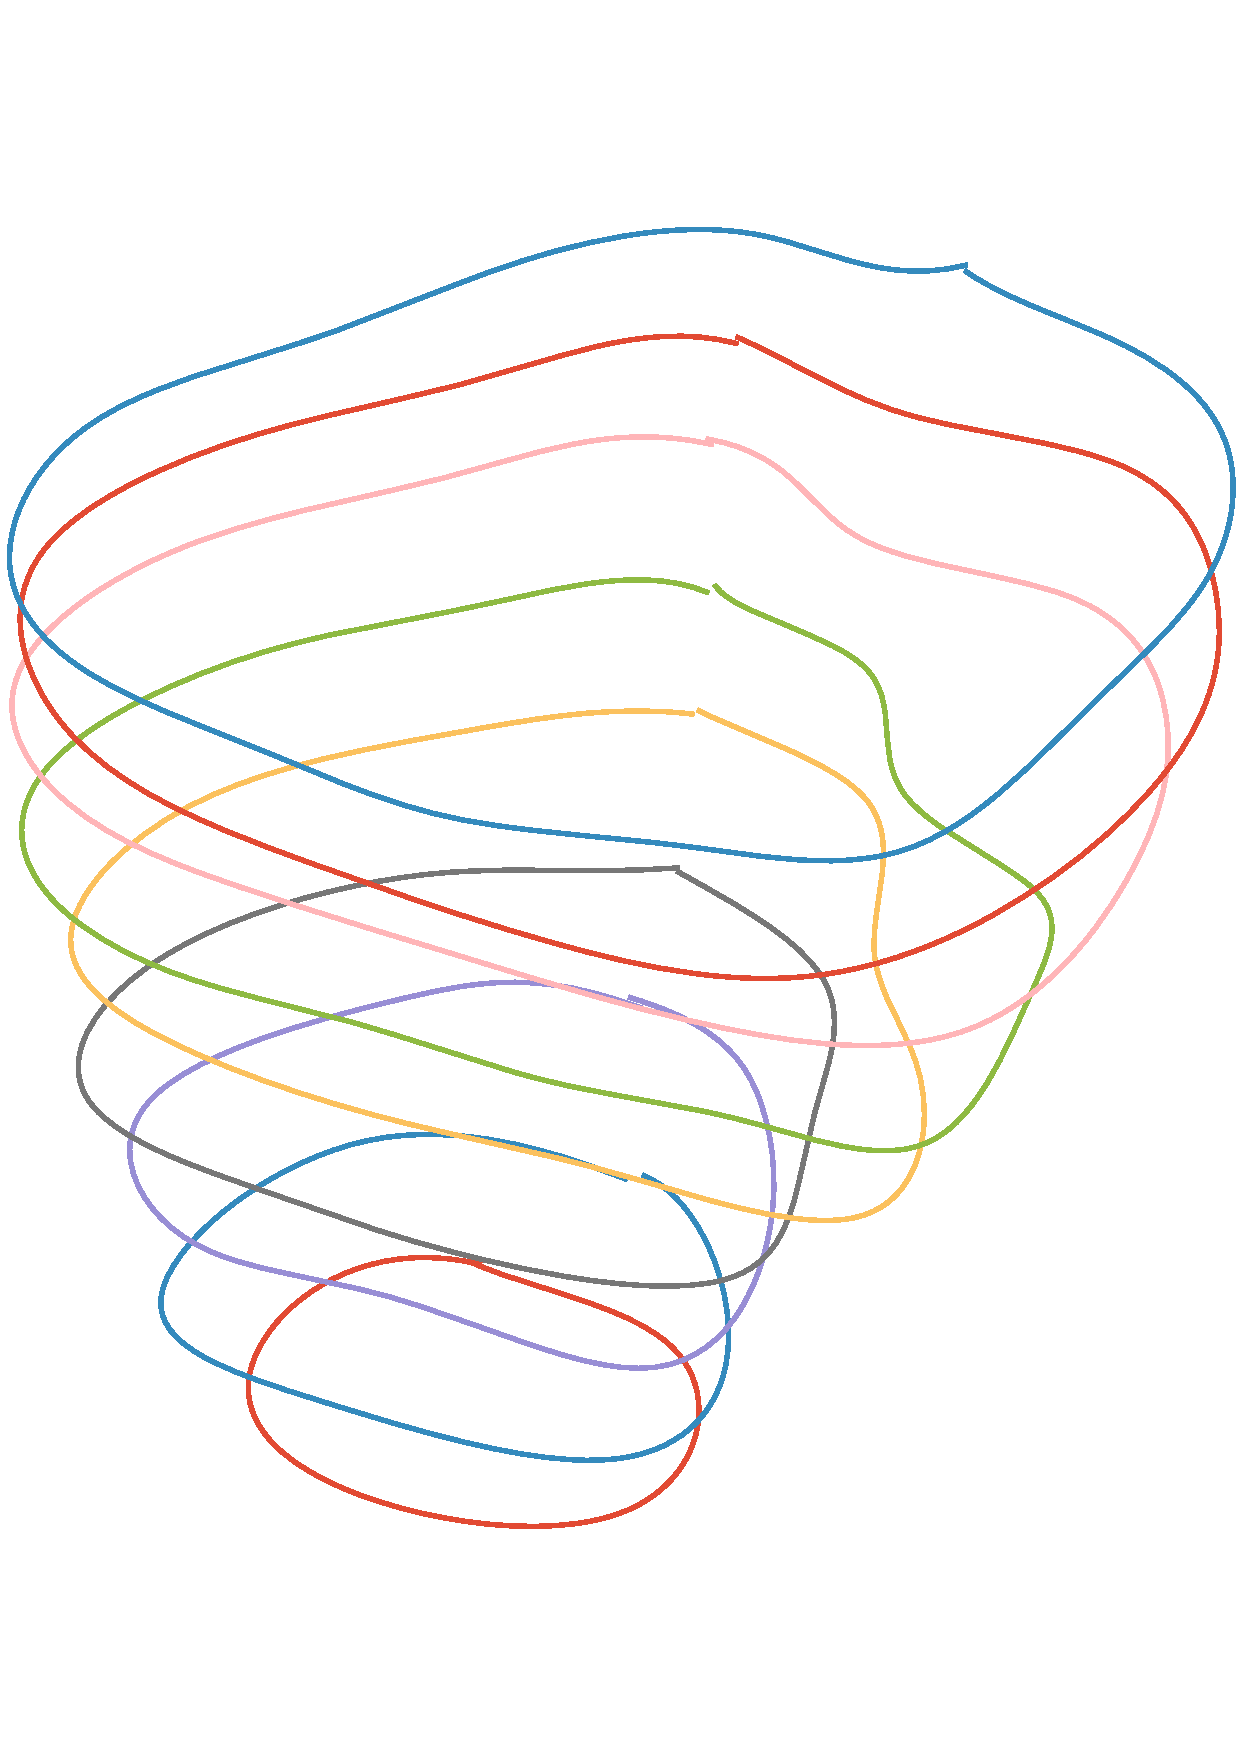
\includegraphics[width=\linewidth]{../images/curves_lambda_5_cropped.pdf}
        \caption{\( \lambda = 5 \% \)}
    \end{subfigure}
    \begin{subfigure}{0.32\textwidth}
        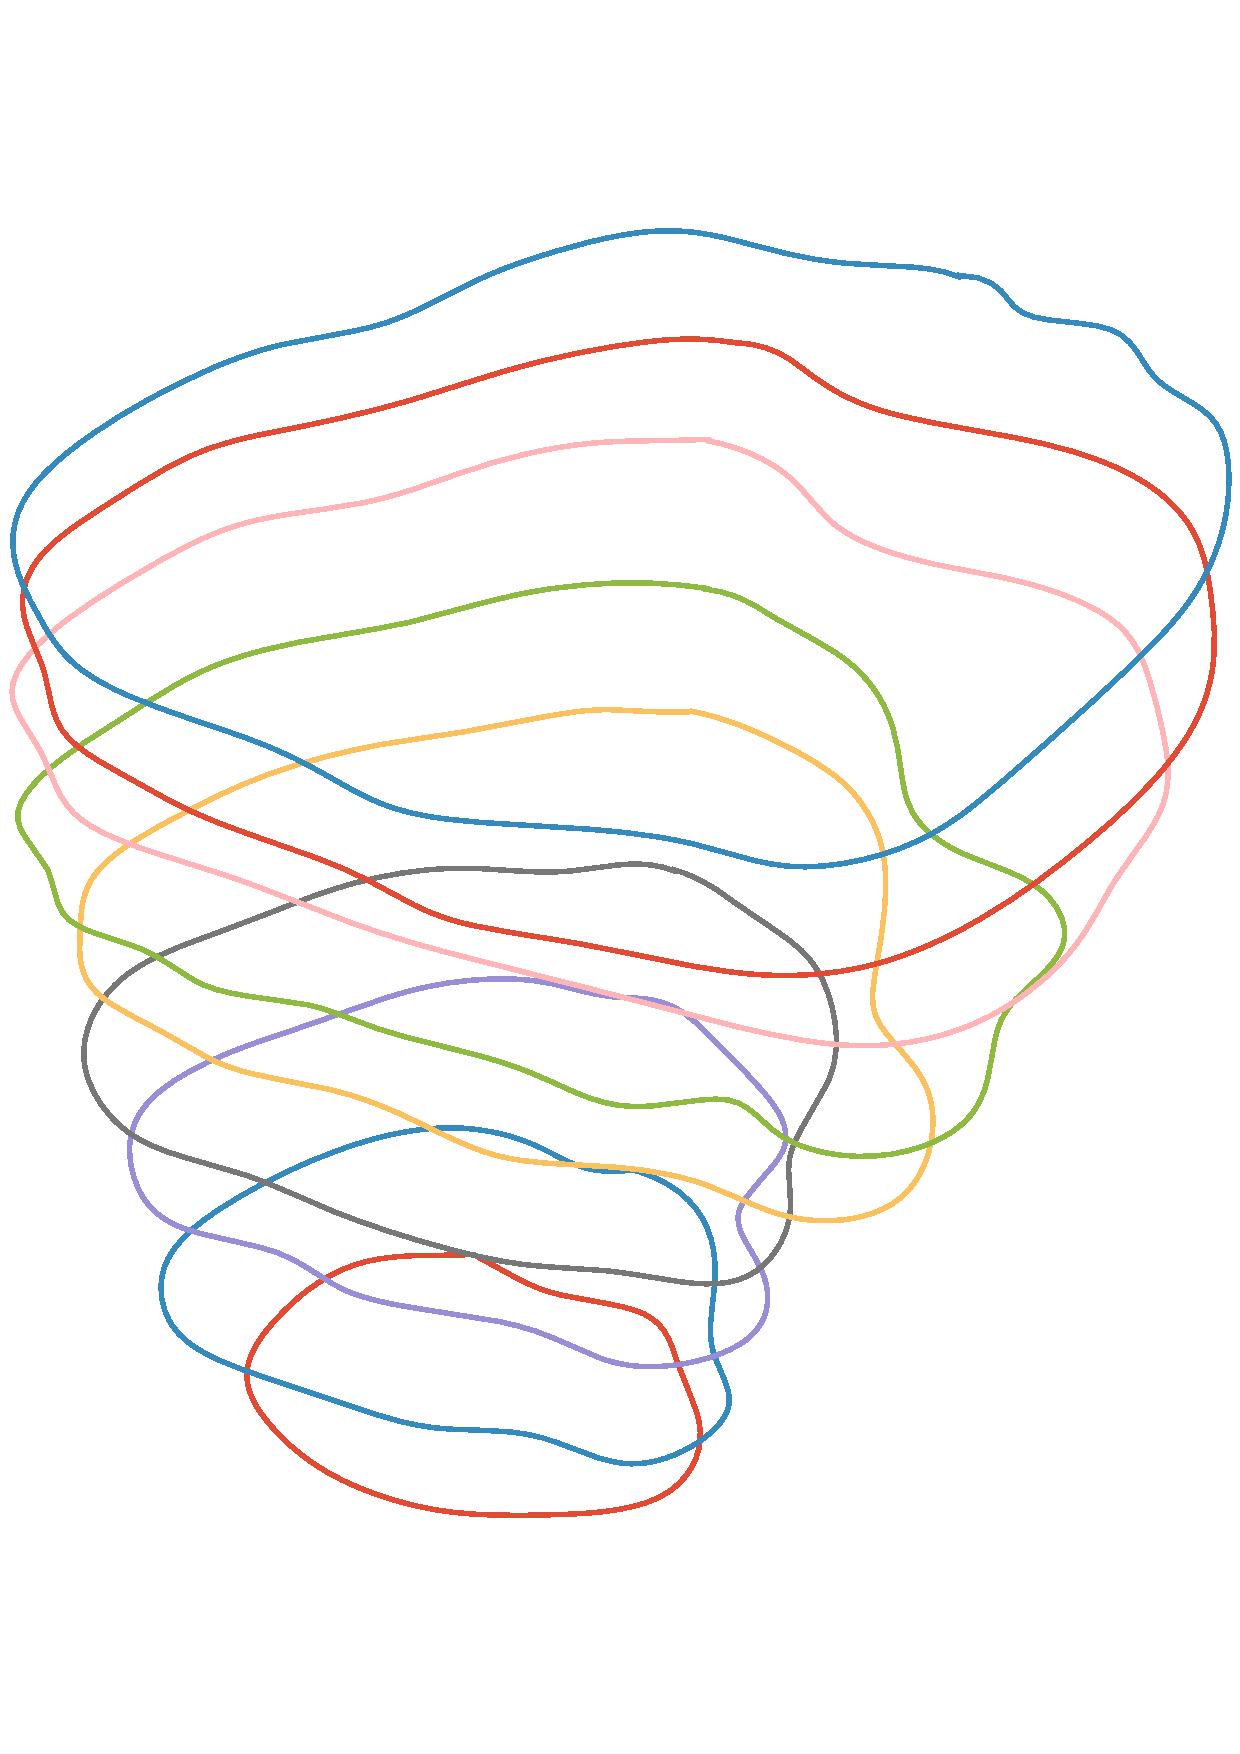
\includegraphics[width=\linewidth]{../images/curves_lambda_10_cropped.pdf}
        \caption{\( \lambda = 10 \% \)}
    \end{subfigure}
    \begin{subfigure}{0.32\textwidth}
        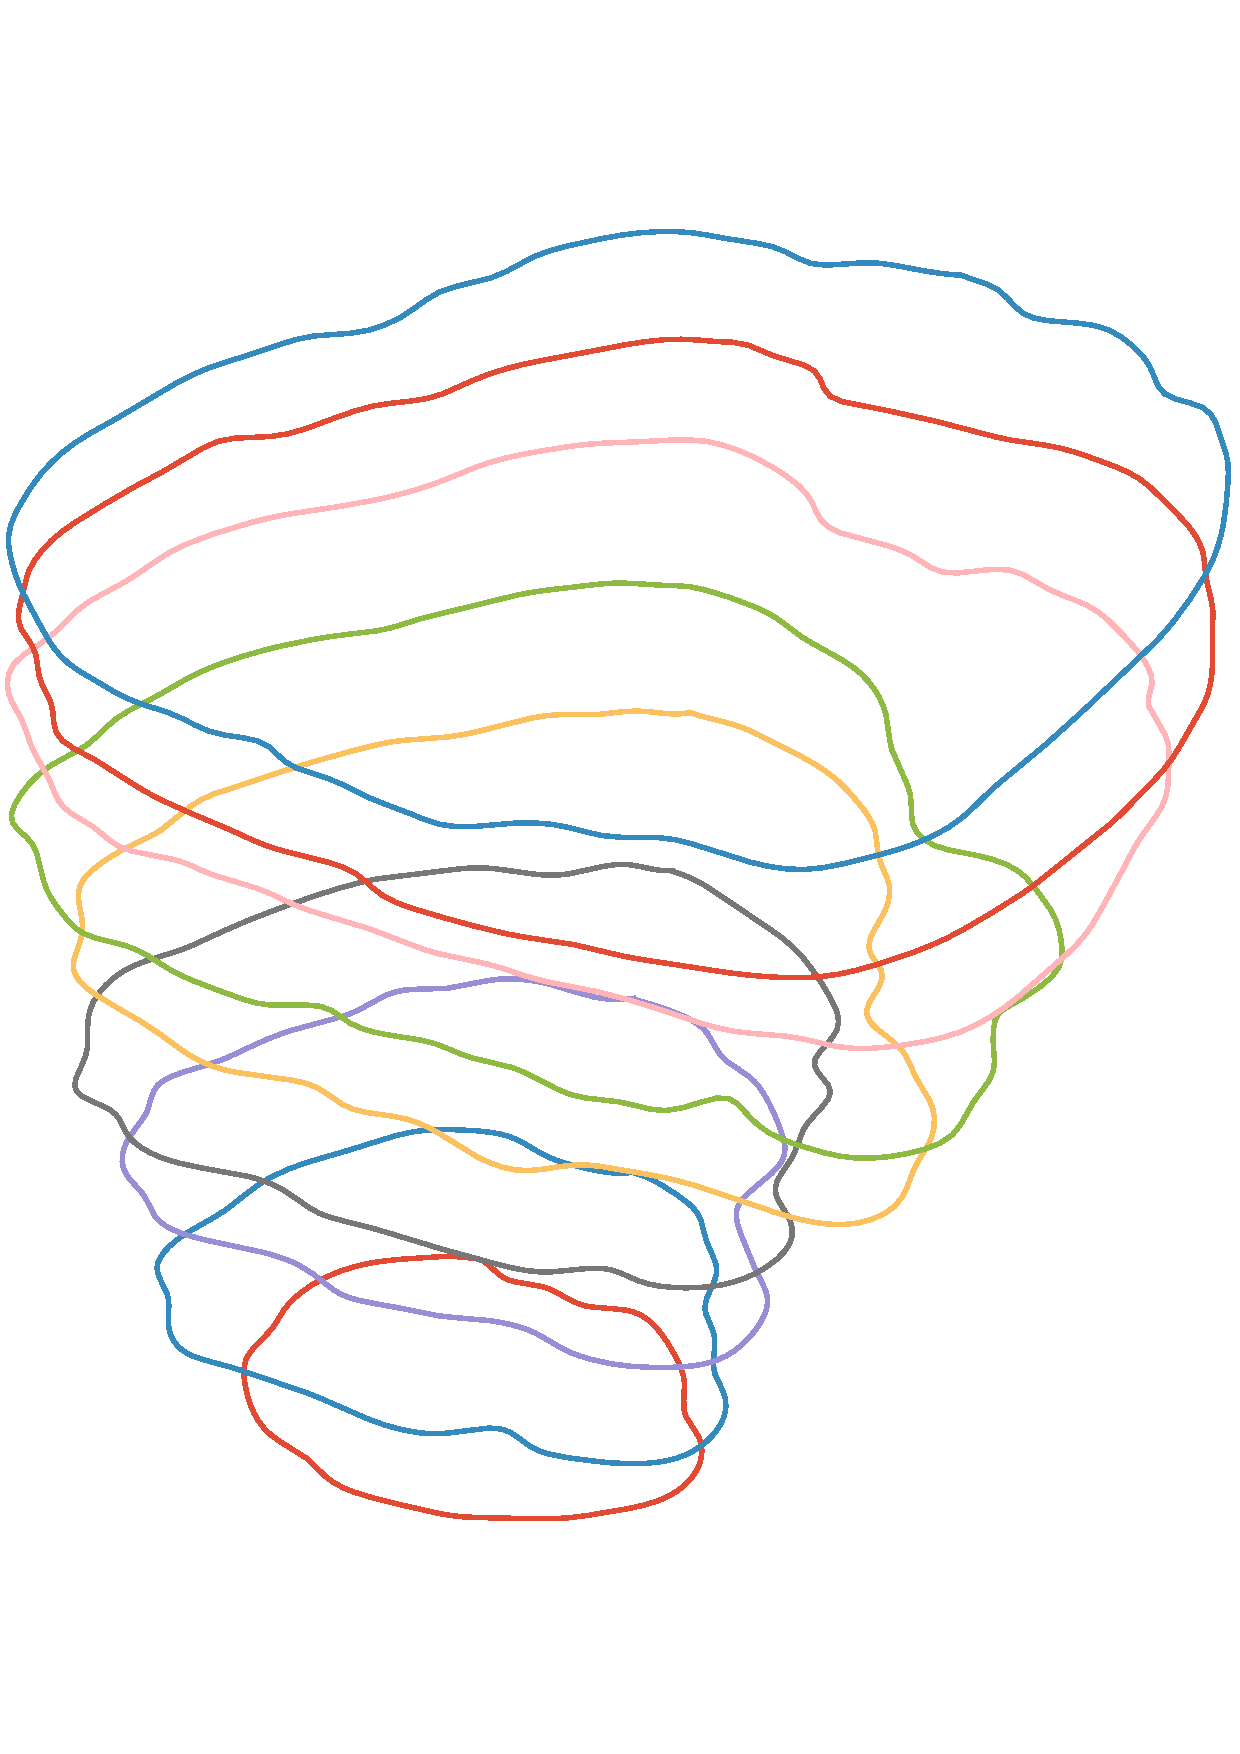
\includegraphics[width=\linewidth]{../images/curves_lambda_20_cropped.pdf}
        \caption{\( \lambda = 20 \% \)}
    \end{subfigure}
    \caption{The least square spline approximations to the nine contour data
    sets for varying number of basis splines as indicated by the parameter \(
    \lambda \). As we can see, more fine scaled structured is preserved for higher
    values of \( \lambda \).}
    \label{fig:contours}
\end{figure}

\chapter{Tensor product spline representation of heart}
\label{cha:tensor_product_spline_representation_of_heart}

In order to find a least squares tensor product spline surface approximating
the data, we first need to construct a data set suitable for approximation.
Having already found the splines \( f_j \) for the contour curves, we can
sample these in order to create a data set of the form \( \x_{i, j} \coloneqq
(x_{i, j}, y_{i, j}, z_{i, j})\) for \(i = 1, \dots, m \) and \(j = 1, \dots, n
\) where \(m\) and \(n\) denote the number of samples in each ``direction''.
From such a data set it is possible to compute the least squares spline surface
\( \f(u, v) \).

\paragraph{Sampling the spline curves:}

Having only nine spline curves \( f_j \) where the \( z \)-component is
constant for fixed \( j \), we can only hope to have at most nine samples
\emph{across} the curves. This means that \( n = 9\). When it comes to sampling
\emph{along} the curves, we can choose more freely. In this assignment we let
\( m = 20 \). This choice immediately puts a constraint on the dimension of the
spline spaces we are allowed to consider, as we require the number of basis
splines in each direction to be no more than the number of data points in each
direction.

Assuming now that the \(j\)th spline \( f_j \) has parameter domain \([0,
u_j]\), we sample \( m \) uniformly spaced points along the curve. This can be
achieved by the following rule:
\begin{equation}
    \notag
    \x_{i, j} \coloneqq f_j(u_j \cdot i / (m - 1))
\end{equation}
for \(i = 0, \dots, m-1\), and then repeating this for each spline \(f_1,
\dots, f_9\).

\paragraph{Parametrization:}

Since we sampled the data points \( \x_{i, j} \) points uniformly along the
curves, it would seem reasonable to also parametrize the rectangular data using
uniform parametrization. Setting \( \mu = 0 \) in the parametrization routine
from above, and normalizing the parameters to the interval \([0, 1]\) we obtain
the parametrization rule \((u_i, v_j) = (i / 19, j / 8)\).

\paragraph{Determining the spline space \(\S_u \otimes \S_v\):}
We now have everything we need to choose the knot vectors. In order to obtain
non-singular collocation matrices, we need to satisfy the
\emph{Schoenberg-Whitney} conditions. This amounts to choosing knots so that
the support of each basis spline contains at least one parameter point.  We
decide on the knot vectors
\begin{align*}
    \tu \coloneqq (0, 0, 0 , 0, \overbrace{\dots}^{7}, 1, 1, 1, 1), \\
    \tv \coloneqq (0, 0, 0, 0, \underbrace{\dots}_{1}, 1, 1, 1, 1), 
\end{align*}
with seven and one interior knots respectively. This ensures that our
univariate spline spaces that make up the tensor product spline space has
dimensions 11 and 5 respectively. The tensor product spline surfaces have been
visualized and can be seen in \cref{fig:surfaces}.
\begin{figure}[htbp]
    \centering
    \begin{subfigure}{0.32\textwidth}
        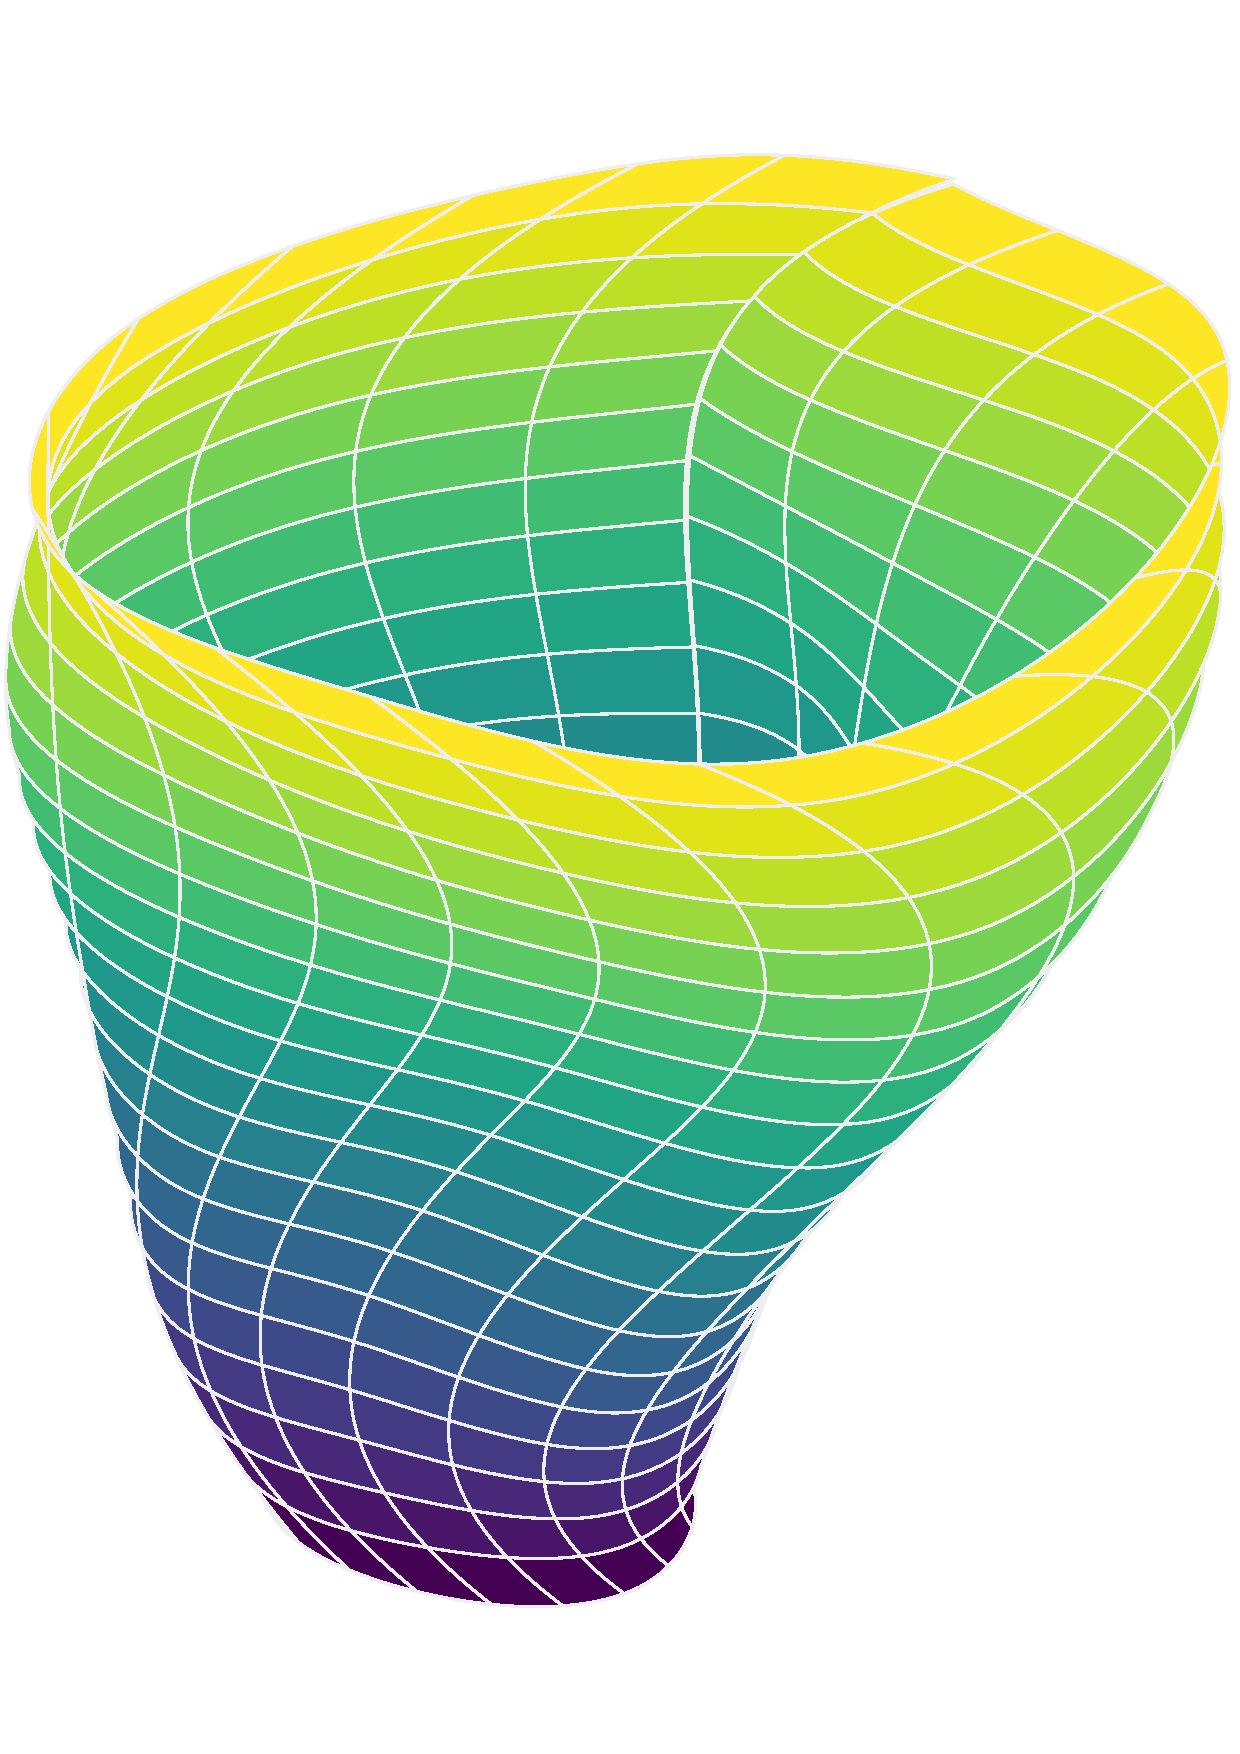
\includegraphics[width=\linewidth]{../images/surfaces_lambda_5_cropped.pdf}
        \caption{\( \lambda = 5 \% \)}
    \end{subfigure}
    \begin{subfigure}{0.32\textwidth}
        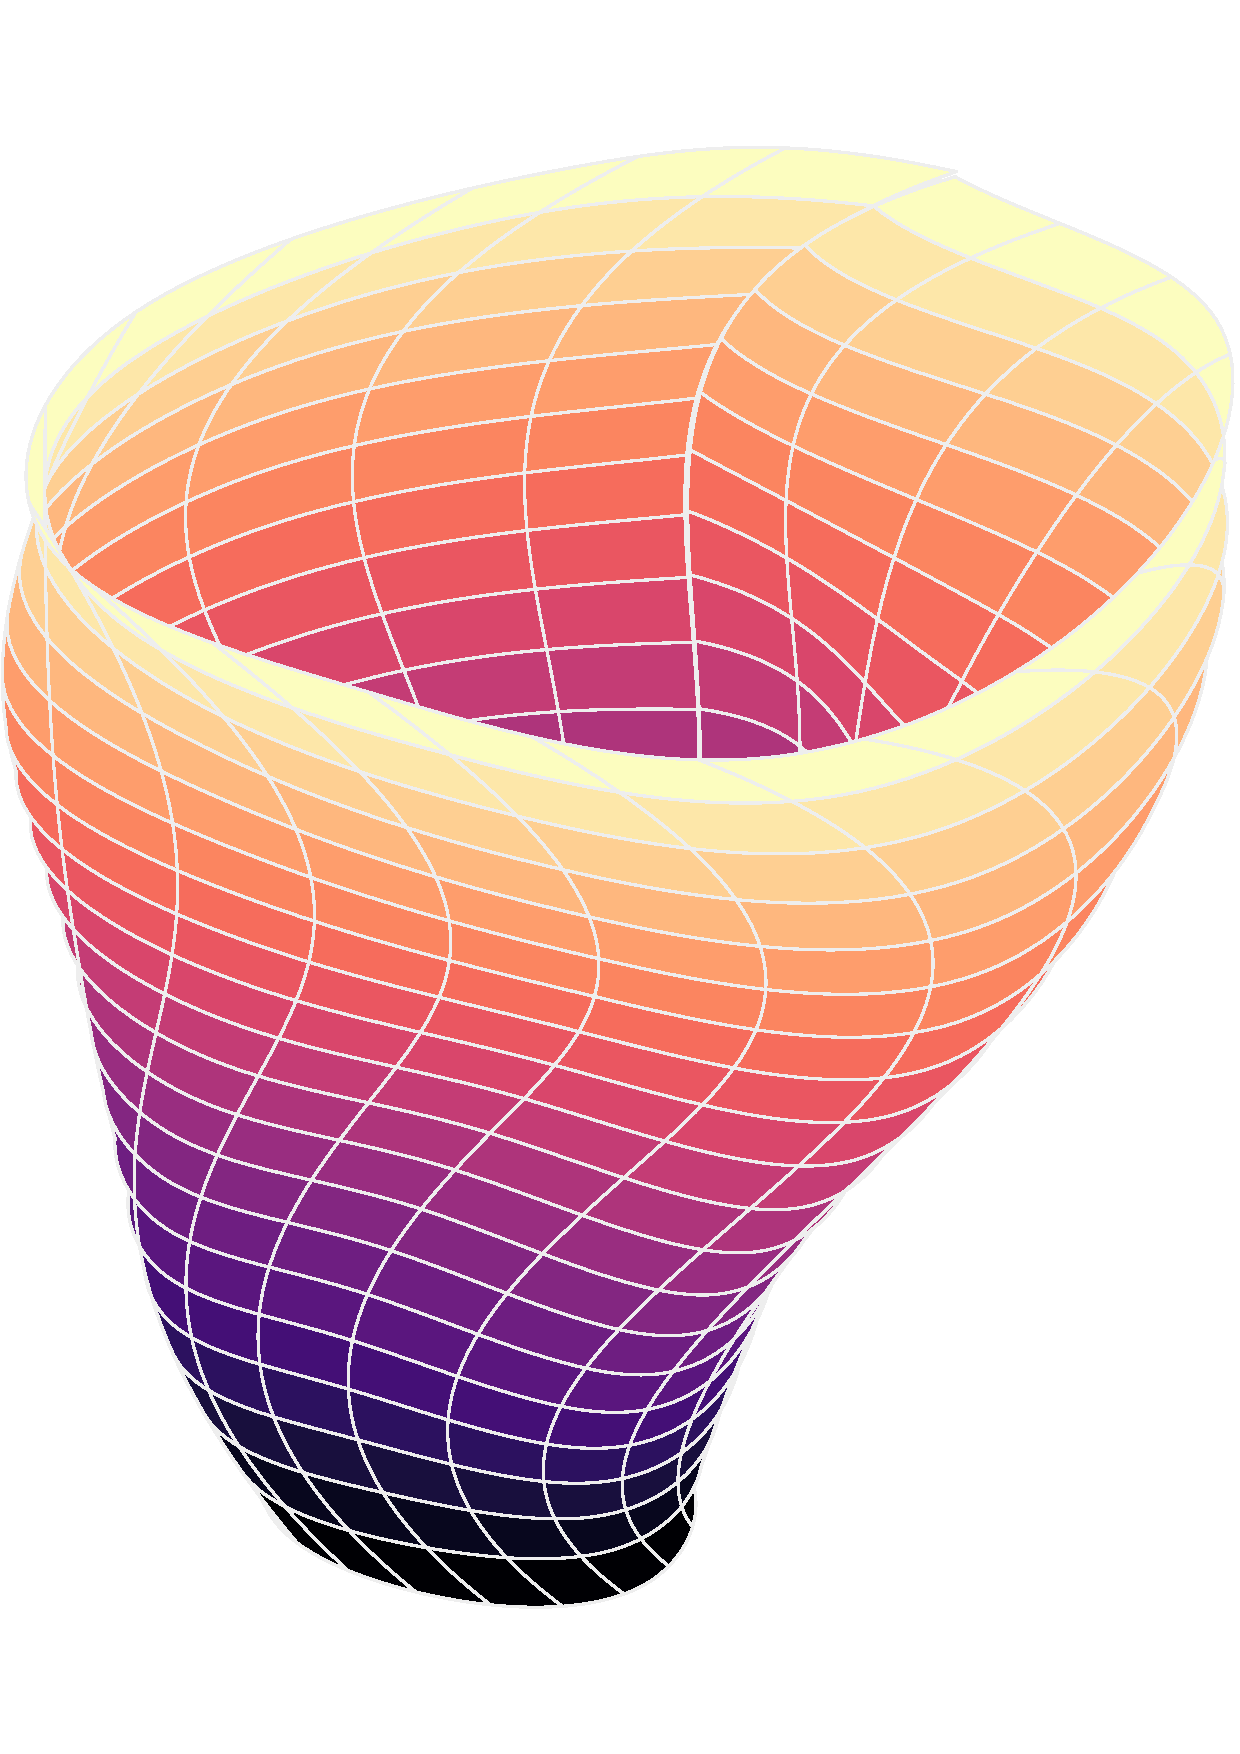
\includegraphics[width=\linewidth]{../images/surfaces_lambda_10_cropped.pdf}
        \caption{\( \lambda = 10 \% \)}
    \end{subfigure}
    \begin{subfigure}{0.32\textwidth}
        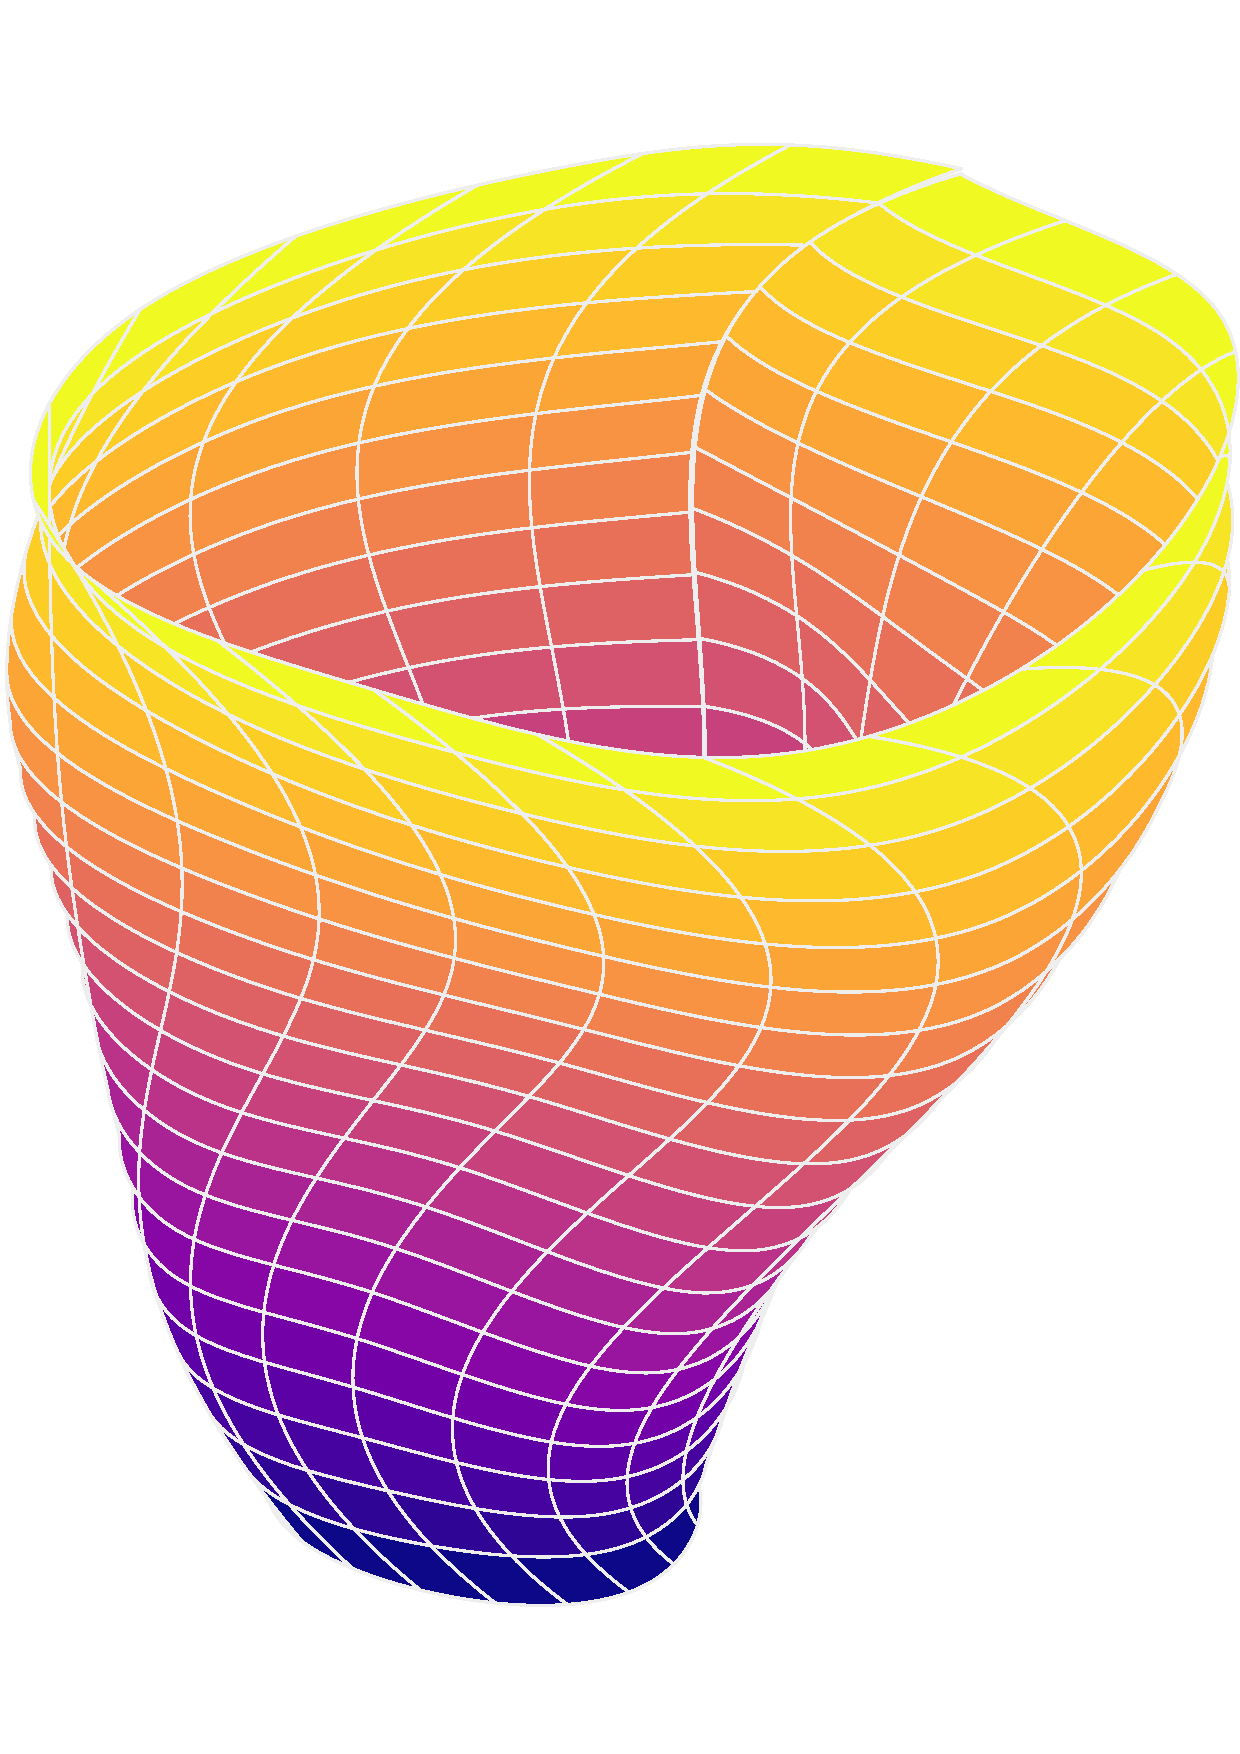
\includegraphics[width=\linewidth]{../images/surfaces_lambda_20_cropped.pdf}
        \caption{\( \lambda = 20 \% \)}
    \end{subfigure}
    \caption{The least square approximating surface \( \f(u, v) \) to the rectangular heart
        data set. Due to the rectangular data relying on the least square
        approximations to the original contour data, we see that the fine
        scaled structure is lost. It therefore seems that there is no real
    benefit to choosing a particularity high \( \lambda \) when it comes to
    modelling purposes.}
    \label{fig:surfaces}
\end{figure}

\clearpage
\appendix
\chapter{Implementation}

During this spline course I have been tinkering on a small
\textsc{Python}-library, opportunistically named \textsc{SEAL} (SplinE
Algorithm Library). It provides high level methods for computing with splines,
and I have employed this during this assignment. The library revolves around
two objects: \texttt{SplineSpace} and \texttt{SplineFunction}. SplineSpaces can
be instantiated with a spline degree \texttt{p} and a knot vector \texttt{t}.
An example of least squares approximation of data of the same form as the
contour data from above is given following:

\begin{enumerate}[I)]
    \item We first load and parametrize the data:
\begin{minted}{python}
import SEAL
import numpy as np

curve = np.loadtxt('hj1.dat')
u = SEAL.parametrize(curve, data_type='curve') 
\end{minted}
\item We can now define our desired spline space, by specifiying a degree, knot end
points, and the desired dimension:
\begin{minted}{python}
p = 2
n = 30
t = SEAL.create_knots(u[0], u[-1], p, n)
S = SEAL.SplineSpace(p, t)
\end{minted}
\item We can now find the least squares approximation in the spline space \texttt{S},
and evaluate it over the knot vector \texttt{t}.
\begin{minted}{python}
f = SEAL.least_squares_spline_approximation(u, curve, S)
t_values = S.parameter_values(resolution=100)
f_values = f(t_values)
\end{minted}
\item The plotting of the spline, its control polygon, and the initial data can now
easily be done:
\begin{minted}{python}
import matplotlib.pyplot as plt
from mpl_toolkits.mplot3d import Axes3D
fig = plt.figure()
axs = Axes3D(fig)
axs.plot(*zip(*f_values))
axs.plot(*zip(*f.control_polygon))
axs.scatter(*zip(*f.control_polygon))
axs.scatter(*zip(*curve))
plt.show()
\end{minted}
\end{enumerate}
The result is shown in \cref{fig:implementation_example}.  The workflow is
completely analogous for tensor product surfaces, and methods for computing
interpolants and variation diminishing spline approximation are also
implemented, both for scalar and parametric splines.
\begin{figure}[htbp]
    \centering
    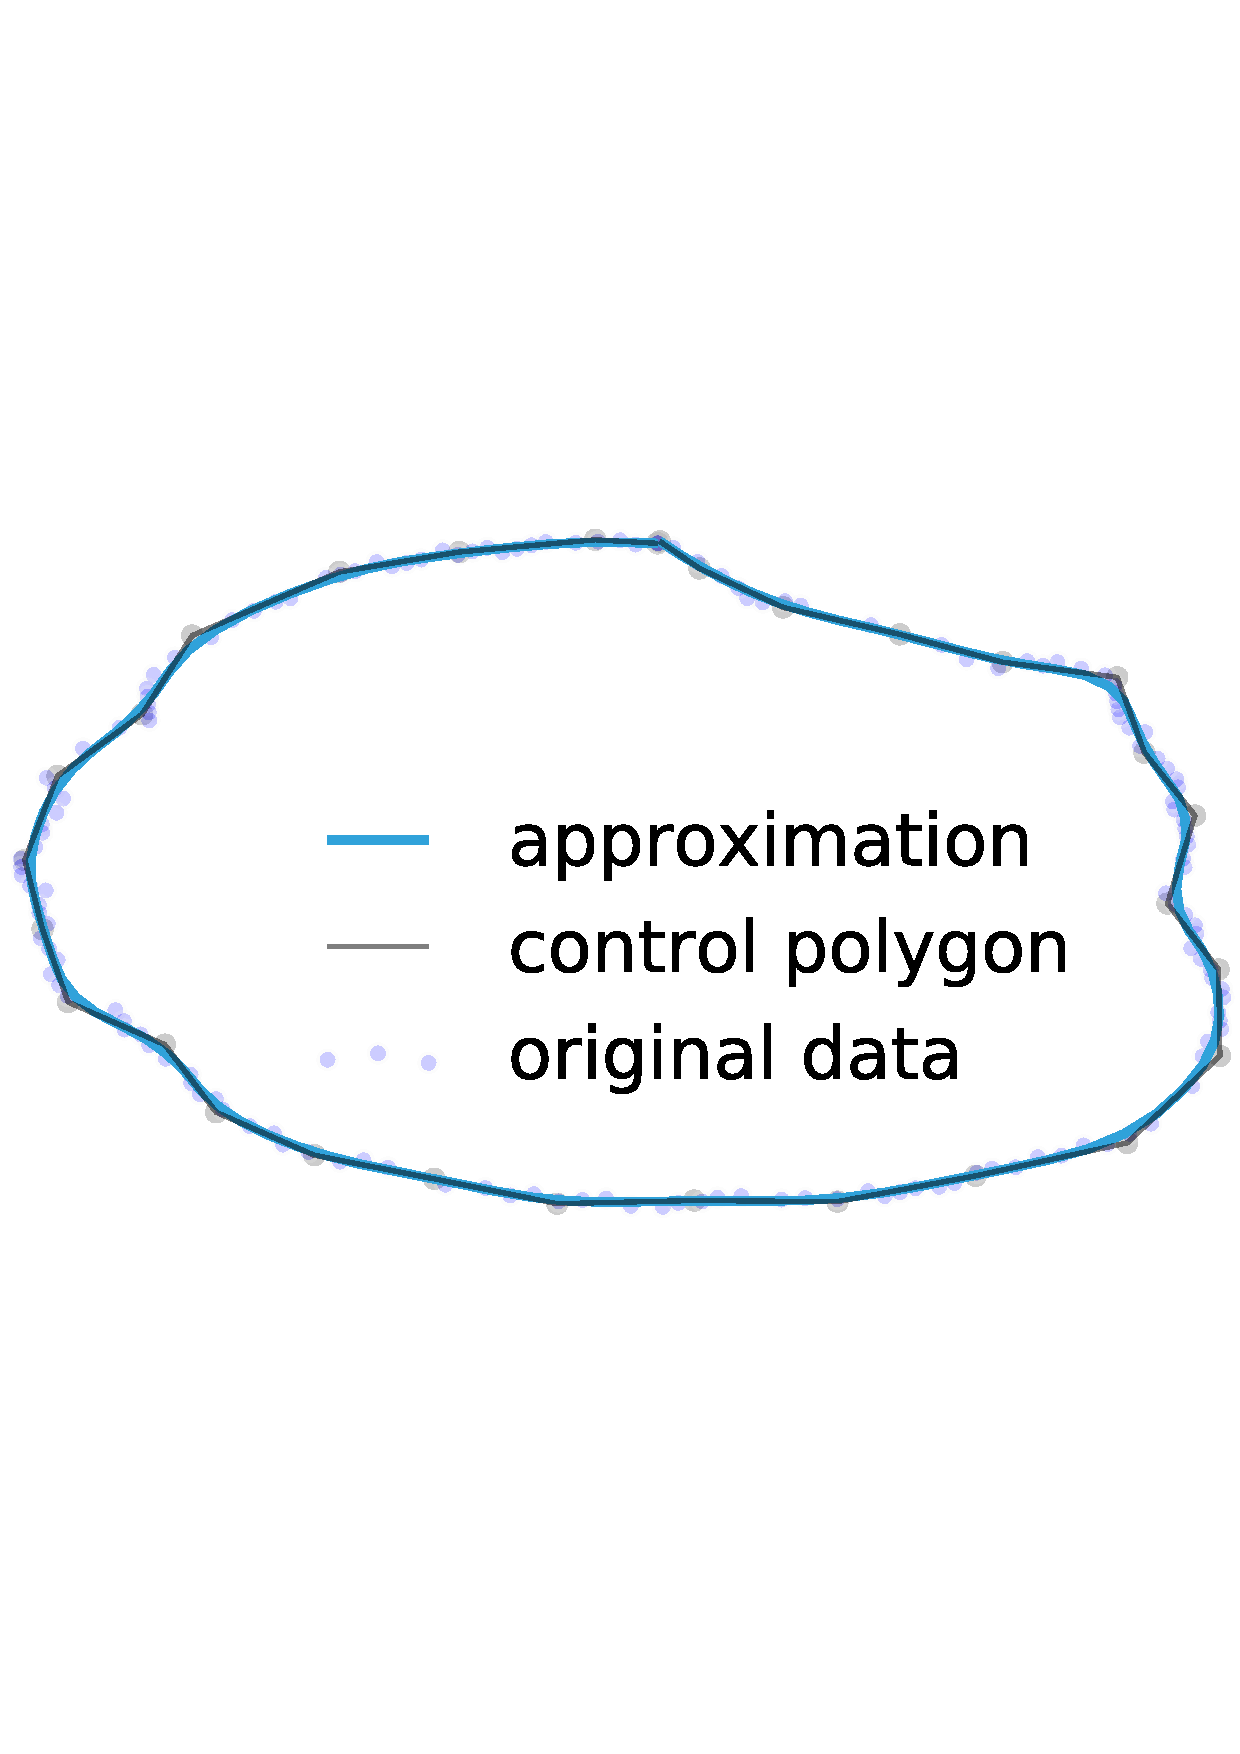
\includegraphics[width=\linewidth]{../images/example_cropped.pdf}
    \caption{The least square approximation to the first contour data set. Here
    visualized with the control polygon and the original data points.}
    \label{fig:implementation_example}
\end{figure}

\end{document}
